\documentclass[a4paper, 11pt]{scrartcl}


\makeatletter
\DeclareOldFontCommand{\rm}{\normalfont\rmfamily}{\mathrm}
\DeclareOldFontCommand{\sf}{\normalfont\sffamily}{\mathsf}
\DeclareOldFontCommand{\tt}{\normalfont\ttfamily}{\mathtt}
\DeclareOldFontCommand{\bf}{\normalfont\bfseries}{\mathbf}
\DeclareOldFontCommand{\it}{\normalfont\itshape}{\mathit}
\DeclareOldFontCommand{\sl}{\normalfont\slshape}{\@nomath\sl}
\DeclareOldFontCommand{\sc}{\normalfont\scshape}{\@nomath\sc}
\makeatother


\usepackage{mathptmx}
\usepackage{anyfontsize}
\usepackage{t1enc}
\usepackage[german]{babel} %choose your language
\usepackage[portrait, margin=1cm]{geometry}
\usepackage[utf8]{inputenc}
\usepackage[dvipsnames]{xcolor}
\usepackage{amscd, amsmath, amssymb, blindtext, empheq, enumitem, multicol, parskip}
\usepackage{graphicx}
\usepackage{tikz}
\usepackage{esint}
\usepackage{wrapfig}
\usepackage{setspace}
\usepackage{trfsigns}

% make document compact
\usepackage[compact]{titlesec}
\titlespacing{\section}{0pt}{*0}{*0}
\titlespacing{\subsection}{0pt}{*0}{*0}
\titlespacing{\subsubsection}{0pt}{*0}{*0}

\parindent 0pt
\pagestyle{empty}
\setlength{\unitlength}{1cm}
\setlist{leftmargin = *}
% Set the color of your style
% Avaiable are: Apricot, Aquamarine, Bittersweet, Black, Blue, blue, BlueGreen, BlueViolet, BrickRed, Brown, BurntOrange, CadetBlue, CarnationPink, Cerulean, CornflowerBlue, Cyan, Dandelion, DarkOrchid, Emerald, ForestGreen, Fuchsia, Goldenrod, Gray, Green, GreenYellow, JungleGreen, Lavender, ... (more at: http://en.wikibooks.org/wiki/LaTeX/Colors)
\def\StyleColor{Yellow}

\DeclareMathOperator{\rot}{rot}
\DeclareMathOperator{\divg}{div}


% define some colors
\usepackage{color}
\definecolor{section}{RGB}{221,95,50}
\definecolor{subsection}{RGB}{221,95,50}
\definecolor{subsubsection}{RGB}{225,157,41}
\definecolor{titletext}{RGB}{0,0,0}
\definecolor{formula}{RGB}{220,230,255}

% section color box
\setkomafont{section}{\mysection}
\newcommand{\mysection}[1]{%
    \Large\sf\bf%
    \setlength{\fboxsep}{0cm}%already boxed
    \colorbox{section}{%
        \begin{minipage}{\linewidth}%
            \vspace*{2pt}%Space before
            \leftskip2pt %Space left
            \rightskip\leftskip %Space right
            {\color{titletext} #1}
            \vspace*{1pt}%Space after
        \end{minipage}%
    }}
%subsection color box
\setkomafont{subsection}{\mysubsection}
\newcommand{\mysubsection}[1]{%
    \normalsize \sf\bf%
    \setlength{\fboxsep}{0cm}%already boxed
    \colorbox{subsection}{%
        \begin{minipage}{\linewidth}%
            \vspace*{2pt}%Space before
            \leftskip2pt %Space left
            \rightskip\leftskip %Space right
            {\color{titletext} #1}
            \vspace*{1pt}%Space after
        \end{minipage}%
    }}
    
%subsection color box
\setkomafont{subsubsection}{\mysubsubsection}
\newcommand{\mysubsubsection}[1]{%
    \normalsize \sf\bf%
    \setlength{\fboxsep}{0cm}%already boxed
    \colorbox{subsubsection}{%
        \begin{minipage}{\linewidth}%
            \vspace*{2pt}%Space before
            \leftskip2pt %Space left
            \rightskip\leftskip %Space right
            {\color{titletext} #1}
            \vspace*{1pt}%Space after
        \end{minipage}%
    }}    
%subsection color box
\title{DC-Netzwerke}
\author{www.n.ethz.ch/$\sim$zrene/nus1/nus1.html}
\date{}

\newcommand{\dis}[1]{\hspace{#1cm}}
    
% equation box        
\newcommand{\eqbox}[1]{\fcolorbox{section}{formula}{\hspace{0.5em}$\displaystyle#1$\hspace{0.5em}}}

%macro for vectors 
%\newcommand{\vect}[1]{\vec{#1}}
\newcommand{\vect}[1]{\boldsymbol{#1}}

%\renewcommand{\familydefault}{cmss}
\DeclareSymbolFont{letters}{OML}{ztmcm}{m}{it}
\DeclareSymbolFontAlphabet{\mathnormal}{letters}
%\everymath{\displaystyle}  %bigger equations
\begin{document}
%\setcounter{secnumdepth}{0} %no enumeration of sections
		\maketitle
		\setcounter{section}{3}
				\begin{multicols*}{2}

						\subsection{Spannungs- und Stromquellen}
				\begin{itemize}
					\item \textbf{Ideale Quellen:}\\
					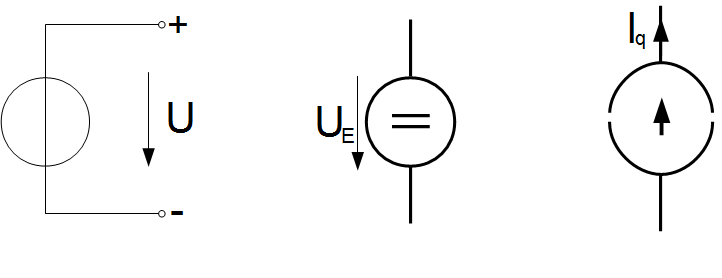
\includegraphics[scale=0.2]{source/quellen.png}
					$\rightarrow$ Keine Verlustleistung
					%\item \textbf{Leistung:} $P=UI=RI^2=\frac{U^2}{R}$
					\item \textbf{Reale Stromquelle} Leerlaufspannung: $U_0=R_i\cdot I_0$
					\item \textbf{Reale Spannungsquelle} Kurzschlussstrom: $I_K=\frac{U_0}{R_i}$
					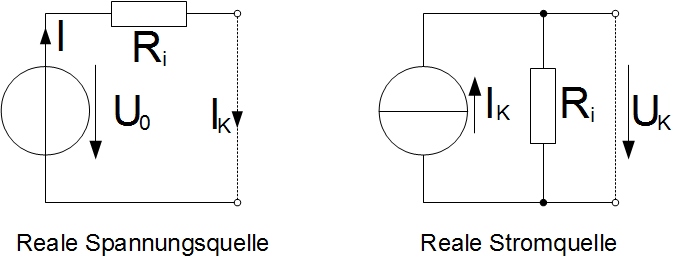
\includegraphics[scale=0.25]{source/realeQuellen.png}\\
					\textit{Umwandlung:} $_{[U-Quelle]}\,U_0=R_i\cdot I_0 \, _{[I-Quelle]}$
					\item \textbf{Kirchhoff'sche Maschenregel:} $\sum_{Masche}U_k=0$
					\item \textbf{Kirchhoff'sche Knotenregel:} $\sum_{Knoten}I_k=0$
					\item \textbf{Leistungsanpassung}\\
				Die Leistung wird maximiert, wenn gilt: \eqbox{R_L=R_i}
				\end{itemize}
				
				\textbf{Wechselwirkung Quelle $\Leftrightarrow$ Verbraucher}
				\begin{itemize}
					\item Gleichmässige Energieabgabe ist nur bei identischen Quellen möglich.
					\item Leistungsabgabe von zusammengeschalteten Spannungsquellen ist unterschiedlich, wenn sie über versch. $R_i$ oder $U_L$ verfügen.
					\item Quellen können zu \textit{Verbrauchern} werden.			
				\end{itemize}
				
				\subsection{Einfache Netzwerkberechnungen}
				\begin{tabular}{ll}
					\textbf{[R] Seriell:} &$R_{ges}=\sum\limits_{k=1}^{n}{R_k}$\\
					\textbf{[R] Parallel:} &$\frac{1}{R_{ges}}=\sum\limits_{k=1}^{n}{\frac{1}{R_k}}$ \quad $n=2\rightarrow R_{ges}=\frac{R_1R_2}{R_1+R_2}$\\
					\textbf{[C] Seriell:} &$\frac{1}{C_{ges}}=\sum\limits_{k=1}^{n}{\frac{1}{C_k}}$ \quad $n=2\rightarrow C_{ges}=\frac{C_1C_2}{C_1+C_2}$\\
					\textbf{[C] Parallel:} &$C_{ges}=\sum\limits_{k=1}^{n}{C_k}$\\
					\textbf{[L] Seriell:} &$L_{ges}=\sum\limits_{k=1}^{n}{L_k}$\\
					\textbf{[L] Parallel:} &$\frac{1}{L_{ges}}=\sum\limits_{k=1}^{n}{\frac{1}{L_k}}$ \quad $n=2\rightarrow L_{ges}=\frac{L_1L_2}{L_1+L_2}$				
				\end{tabular}

				\subsection{Spannungs-/Stromteiler}
				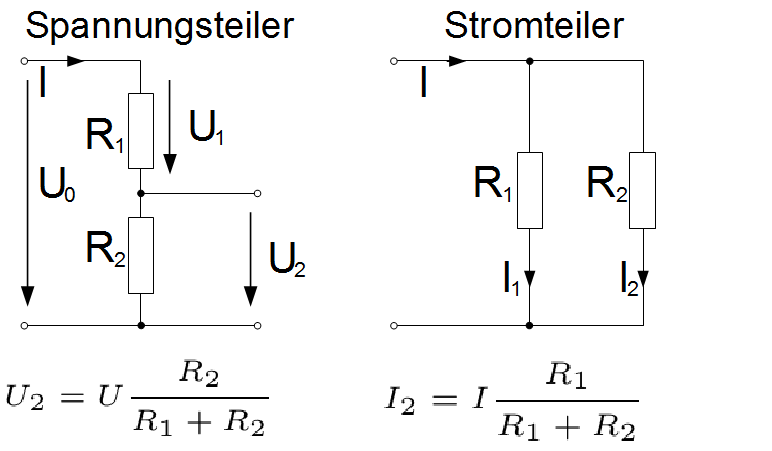
\includegraphics[scale=0.24]{source/teiler.png}\\\\
				\textbf{Belasteter Spannungsteiler:}\\
				$$R_{2}'=\frac{R_2R_L}{R_2+R_L}\rightarrow \frac{U_2}{U}=\frac{R_{2}'}{R_1+R_{2}'}=\frac{R_2R_L}{R_1(R_2+R_L)+R_2R_L}$$

				\subsection{Wirkungsgrad}
				$$\eta=\frac{P_L}{P_{ges}}\cdot 100\%=\frac{I^2R_L}{I^2(R_i+R_L)}\cdot 100\%=\frac{R_L/R_i}{1+R_L/R_i}\cdot 100\%$$
				Umgeformt (1-140): $\eta=\left(1-\frac{I}{I_{max}}\right)\cdot 100\%$\\

				Bei der Leistungsanpassung beträgt der Wirkungsgrad $50\%$.\\
				\subsection{Widerstandsmessung (1-131)}
				\begin{itemize}
					\item \textbf{Mit korrekter Spannungsmessung:}\\
					$R=\frac{U_R}{I_R}=\frac{U_V}{I_A-I_V}=\frac{U_V}{I_A-U_V/R_V}=\frac{U_VR_V}{I_AR_V-U_V}$
					\item \textbf{Mit korrekter Strommessung:}\\
					$R=\frac{U_R}{I_R}=\frac{U_V-U_A}{I_A}=\frac{U_V-R_AI_A}{I_A}$
				\end{itemize}

				\subsection{Superpositionsprinzip}
				Für jede Quelle das Netzwerk analysieren, die Anderen ausschalten, Resultate addieren.
				\begin{itemize}
					\item Spannungsquellen $\rightarrow$ Kurzschliessen
					\item Stromquellen $\rightarrow$ Leerlauf
				\end{itemize}				


		\end{multicols*}

\setcounter{secnumdepth}{2}
\end{document}
